\chapter{Winning SBIR Contracts}

This lecture is about the interval before traction: the awkward, expensive region where a technical invention is real enough to matter, but not yet reduced to a product that customers can buy, test, or even fully understand. Steve Derezinski presents SBIR not as a magic pool of government cash, and not as a form-filling exercise, but as a funding instrument with a particular logic: incentives, deadlines, agency variation, eligibility rules, and compliance obligations. The lecture belongs in the practical sequence of \emph{Nuts and Bolts of New Ventures}, credited to Joseph Hadzima and MIT OpenCourseWare, with this edition curated by LazyingArt LLC through Video2Book.

\section{Why This Lecture Exists}

The opening promise is deliberately attractive: free government money. But almost immediately the lecture narrows the claim. The subject is not how to fill out SBIR forms. The subject is how SBIR awards are actually won.

Derezinski explains that he built the lecture because he saw a gap at MIT. There was administrative advice, and there were consultants, but not enough direct discussion of the practical winning process. He then gives the students a small piece of evidence from the prior year: the applicants he knew about won awards, and one company instead raised a \(\$5\) million venture round. That anecdote is not a theorem. It is a way of saying: this topic can matter materially to a young technology company.

His background supplies the operating lens. He was trained as a mechanical engineer at MIT, worked as a roboticist, patented an algorithm for reducing vibration in the space shuttle robotic arm, went through Sloan, helped create a faculty venture studio at Georgia Tech, and later worked in Kendall Square forming companies from technology. The transcript gives two different federal-contract figures, roughly \(\$40\) million and a \(\$23\) million list, so we should not combine them into a single precise number. The safe point is that he has substantial direct experience as a PI or business lead on federal contracts with agencies including NASA, NSF, DOE, ARPA-E, and DOD.

The first rule of the lecture is therefore not about SBIR specifically. It is about money generally:

\begin{equation}
\text{money is not just cash; it is a constraint system.}
\end{equation}

Different money has different color. It brings different motivations, different reporting duties, different time constants, and different failure modes. Once we see that, the rest of the lecture becomes an exercise in matching the stage of the venture to the right kind of money.

\section{Disruptive Technology And The Funding Gap}

The first substantive distinction is between incremental and disruptive technology. If the product is incremental, ordinary customer discovery can work rather directly. We ask customers what they want, and they answer in the coordinates of what they already have: cheaper, faster, higher quality. Their present product gives them the language for the next product.

Disruptive technology has a different problem. Customers may not know what to ask for until they can see it, touch it, test it, or imagine its use. The lecture invokes the familiar examples of the faster horse and of customers who do not know what they want until they are shown. The point is not to celebrate mythology about visionaries. The point is a practical one:

\begin{equation}
\text{disruptive technology}
\quad\Longrightarrow\quad
\text{customer understanding often requires reduction to practice.}
\end{equation}

Now the funding gap appears. Universities and government research programs can support discovery, especially when the application is not yet clear. Private capital can support expansion when a company has customers, traction, and financial history. Between these two regions lies the hard interval: the work needed to turn a paper, laboratory result, or prototype into something the market can evaluate.

\subsection{Question \& Answer}

\paragraph{Question.}
If customers cannot yet understand the product, how can a startup validate or fund it?

\paragraph{Answer.}
The lecture's answer is that we should not pretend that ordinary customer traction already exists. The first task is to reduce the technology to practice far enough that customers can respond intelligently. That is the stage where Derezinski places SBIR-type funding: not as a universal best source of startup capital, but as a practical instrument for deep-technology work before repeat customer traction.

The local obstacle can be written as

\begin{equation}
\text{paper or lab result}
\;\not\Rightarrow\;
\text{customer-ready product}.
\end{equation}

There is a missing middle term: reduction to practice. The lecture argues that this missing term is better matched to grants and non-recourse funding than to recourse capital.

\section{The Research-To-Market Boundary}

The central slide of the lecture turns the funding gap into a stage map. The visible process is

\begin{equation}
\text{Research and inventions}
\rightarrow
\text{Technology Projects}
\rightarrow
\text{Company Projects}
\rightarrow
\text{Funded Company}.
\end{equation}

\begin{figure}
\centering

\includegraphics[width=\linewidth]{lecture_11_figure_02.png}
\caption{Research-to-market funding boundary. The screenshot is the lecture's direct visual evidence for the distinction between technology exploration, customer-focused company execution, and the funding types appropriate on each side of the traction boundary.}
\end{figure}

The two blue boxes carry the lecture's central distinction. A \emph{technology project} is still exploring applications. It may contain serious research, but there is not yet a real customer who understands it, has engaged with it, knows how to buy it, or knows how to interact with it. A \emph{company project} comes later: there is a demo, something people can use, a clearer customer focus, and a need to refine, debug, package, and execute.

The dashed boundary in the slide is not labeled, but the transcript supplies its meaning. It is the boundary between no repeat customer traction and repeat customer traction. A compact reconstruction is:

\begin{figure}
\centering
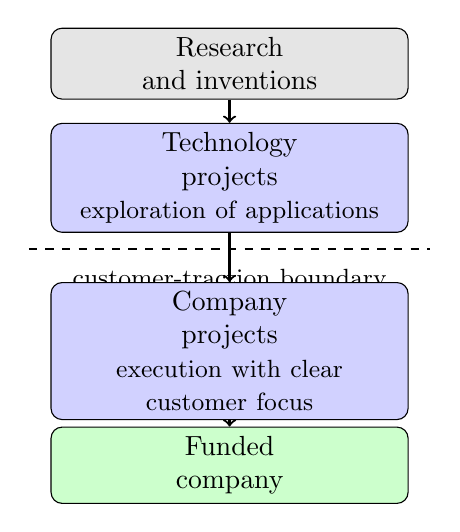
\begin{tikzpicture}[x=1cm,y=1cm]
\node[draw, rounded corners, align=center, text width=4.3cm, minimum height=0.75cm, fill=gray!20] (r) at (0,0)
{Research\\and inventions};

\node[draw, rounded corners, align=center, text width=4.3cm, minimum height=1.05cm, fill=blue!18] (t) at (0,-1.45)
{Technology\\projects\\{\small exploration of applications}};

\draw[dashed, thick] (-2.55,-2.35) -- (2.55,-2.35);
\node[align=center, text width=4.8cm] at (0,-2.75)
{\small customer-traction boundary};

\node[draw, rounded corners, align=center, text width=4.3cm, minimum height=1.05cm, fill=blue!18] (c) at (0,-3.65)
{Company\\projects\\{\small execution with clear customer focus}};

\node[draw, rounded corners, align=center, text width=4.3cm, minimum height=0.75cm, fill=green!20] (f) at (0,-5.10)
{Funded\\company};

\draw[->, thick] (r) -- (t);
\draw[->, thick] (t) -- (c);
\draw[->, thick] (c) -- (f);
\end{tikzpicture}
\caption{A narrow reconstruction of the lecture's research-to-market process for pocket layout.}
\end{figure}

The funding rule is the payload:

\begin{align}
\text{no repeat customer traction}
&\Rightarrow
\text{grants and non-recourse funding},\\
\text{repeat customer traction}
&\Rightarrow
\text{equity, debt, VC, angels, or growth capital}.
\end{align}

This is not a universal law of entrepreneurship. It is a stage map. The warning is strongest on the left side. If we take recourse funding while we are still exploring applications, we create obligations before we know the direction. The company owes performance to somebody, but the market has not yet told us what performance means.

On the right side, the situation changes. When the pump is already working, when customers are present and repeat traction exists, growth capital can be the right fuel. The same dollar can be sensible or dangerous depending on which side of the boundary the company occupies.

\section{Incentives: Why SBIR Is Not Venture Capital}

Once the boundary is in place, the lecture quantifies SBIR. The annual SBIR pool is described as roughly

\begin{equation}
F_{\text{SBIR}}\approx \$4\text{B per year}.
\end{equation}

Derezinski then makes a scale comparison to venture capital. His heuristic is that venture funds deploy about one fifth of committed capital per year. If a government program distributes about \(\$4\) billion per year, the venture-capital-equivalent fund size is

\begin{align}
F_{\text{VC-equivalent}}
&\approx \frac{\$4\text{B}}{1/5}\\
&\approx \$20\text{B}.
\end{align}

This calculation is deliberately simple. Its purpose is not to say that SBIR is venture capital. Its purpose is to make the size visible before we compare incentives.

The lecture then gives the incentive comparison. Angels invest their own money and can decide quickly. Venture capitalists invest limited partners' money, so they are pushed toward high returns, meaningful equity ownership, and time-sensitive exits. The return pressure can be written schematically as

\begin{equation}
\text{VC pressure}
\sim
\text{large return over limited time}.
\end{equation}

If the time stretches, the required financial outcome must become much larger. That is one reason venture capital can be a poor fit for pre-traction technology exploration.

SBIR has a different structure. In the ordinary grant-like sense, the government does not expect repayment. It also does not require the company to become commercially successful in order for the Phase I work to have been legitimate. The expectation is narrower: do the proposed work, use the funds properly, and report the result. Winning an SBIR may later help private diligence, because external investors may treat it as a signal that technically serious reviewers found the work credible. But the SBIR itself is not venture money.

\subsection{Question \& Answer}

\paragraph{Question.}
What is the first motivation of an SBIR program manager?

\paragraph{Answer.}
The class guesses science, job creation, and proper use of funds. Derezinski accepts those as real motivations, but gives the first motivation as: do not get fired.

This is the lecture's clearest tension-and-resolution moment. It explains why the bureaucracy is not merely decorative. If a proposal is excellent but violates an instruction, the program manager may not be able to repair the defect after submission. The safe administrative move is rejection. Thus formality follows from incentives.

We can summarize the practical ordering as

\begin{enumerate}
\item Do not create a compliance problem for the program manager.
\item Do not embarrass the program manager by appearing careless or unserious.
\item Then make the technical case that the work advances the agency's agenda.
\end{enumerate}

This is why instructions, eligibility, formatting, and the official solicitation PDF matter. A proposal is not only a technical argument. It is also evidence that the company can be trusted with public funds.

\section{Agencies, Phases, And Program Shape}

The next movement is from funder incentives to agency architecture. SBIR has one name, but not one uniform implementation. Derezinski notes that NSF says SBIR, while DOD speakers may pronounce it SIBR. The pronunciation is trivial; the underlying lesson is not. Same name, different agency behavior.

He then splits agencies into two practical buckets: market-driven and mission-driven.

\begin{table}
\centering
\small
\begin{tabular}{p{0.27\linewidth}p{0.30\linewidth}p{0.33\linewidth}}
\hline
Agency type & Where the customer sits & Practical implication\\
\hline
Market-driven & Outside the agency, in the marketplace & The proposal must make a credible case that someone will buy, adopt, or validate the technology. NSF and DOE are given as examples.\\
Mission-driven & Inside the agency or its contractor ecosystem & The solicitation may specify a narrow operational need. DOD and NASA are given as examples.\\
\hline
\end{tabular}
\caption{The lecture's operational distinction between market-driven and mission-driven SBIR agencies.}
\end{table}

Market-driven solicitations may sound broad: do something important in optics, energy, software, or another technology area, and show that the market cares. Mission-driven solicitations can be much more specific: a battery with a particular pack constraint, operating temperature, duration, weight, and field condition. The specificity is both burden and opportunity. It is harder to match, but it may also reduce the number of serious competitors.

\subsection{Question \& Answer}

\paragraph{Question.}
Is the market-driven versus mission-driven split just the lecturer's interpretation?

\paragraph{Answer.}
The transcript answers that the framing is tied to America's Seed Fund and NSF material, but the chapter should treat it as an operational taxonomy rather than a statutory classification. It tells founders where to look for the customer, how broad the solicitation may be, and how much matching work the proposal must do.

The phase structure then adds the next layer of operating rules:

\begin{align}
p(\text{Phase I win}) &\approx 10\%\text{--}15\%,\\
p(\text{Phase II win}\mid \text{Phase I completed}) &\approx 50\%.
\end{align}

Phase I is the entry point. One must win Phase I to qualify to apply for Phase II. Phase III is commercialization tracking; in the lecturer's framing, there is no ordinary federal Phase III funding. The exception he emphasizes is a Phase IIb-type matching program.

Let \(P\) be qualifying private recourse investment and \(M(P)\) be the federal match. The lecture states a two-to-one private-to-federal match, capped at \(\$500{,}000\). The compact rule is

\begin{equation}
M(P)=\min\left(\frac{P}{2},\$500{,}000\right).
\end{equation}

The examples are immediate:

\begin{align}
P=\$1{,}000{,}000
&\Rightarrow
M(P)=\$500{,}000,\\
P=\$250{,}000
&\Rightarrow
M(P)=\$125{,}000.
\end{align}

The private investment must be real recourse funding. The lecture explicitly rejects self-loan games: one cannot lend money to oneself, collect the match, and repay oneself. Investor letters and investment structure matter because they prove that the private money is genuine.

Timing also enters here. The federal fiscal year closes on September 30, and a new one begins October 1. Many processes are driven by the need to allocate awards before the year closes, even if some activity spills over. Mission-driven agencies may also use pre-release windows. During those windows, founders may be able to speak more freely with program managers; once the topic is locked down, questions may have to be posted publicly.

\section{Eligibility, Multiple Applications, And SBIR Versus STTR}

Eligibility is not merely a checklist. It is a timing problem. The basic constraints in the lecture are

\begin{align}
\text{employees} &< 500,\\
\text{U.S. citizen or permanent-resident ownership} &\ge 51\%.
\end{align}

The company must be for-profit, and both startups and established companies can apply. Derezinski adds a practical observation from older DOD winner data: one-person companies can win, but the more natural early-company shape is often two to nine people, with some mixture of technical and business capability.

The timing rule is central:

\begin{equation}
\text{eligibility is determined at time of award, not merely at submission.}
\end{equation}

That matters for students, postdocs, and founders still inside a university. One may describe a plan to form or join the company by the time of award, but the team, employment, and budget commitments must become true when the award is made. The PI need not necessarily have a PhD or MD, but must have the technical expertise to oversee the scientific and technical work. On citizenship and visa questions, the lecture is explicitly cautious. The company ownership rule is clear; the PI visa details should not be turned into legal advice.

\subsection{Question \& Answer}

\paragraph{Question.}
Can we apply to multiple agencies, or does that create a duplicate-award problem?

\paragraph{Answer.}
The distinction is the scope of work. If one proposal funds software development and another funds a different technical component of the same eventual product, those may be distinct scopes. If the same work is copied from NIH to DOD with only the agency name changed, that is the problem.

A useful notation is

\begin{equation}
\operatorname{scope}(P_i)=\text{the work actually funded by proposal }P_i.
\end{equation}

The duplicate-award constraint is

\begin{equation}
\operatorname{scope}(P_i)=\operatorname{scope}(P_j)
\quad\Longrightarrow\quad
\text{do not accept both awards.}
\end{equation}

Different scopes may be disclosed and separately pursued. The same work cannot be funded twice. The lecturer treats this not as a clever probability game, but as a compliance boundary. The loose intuition that two \(15\%\) chances may feel like \(30\%\) should not be formalized as independent probability.

\paragraph{Question.}
Do key team members have to be inside the company?

\paragraph{Answer.}
If a person is named, budgeted, and used as part of the credibility of the proposal, then the company must be able to deliver that person at time of award. Generic later hires are different. A budget line for unspecified software developers is not the same as a named expert whose biography helped the proposal win.

\paragraph{Question.}
How should founders handle incorporation and university conflict of interest?

\paragraph{Answer.}
The lecture deliberately does not give a universal answer. Registration often requires some entity or registration path, but university conflict-of-interest issues depend on the lab, department, institution, and technology rights. The right note is caution, not invented legal advice.

The SBIR/STTR distinction adds another layer. SBIR permits a research institution partner; STTR requires one. The lecture gives the allocation arithmetic as follows:

\begin{align}
\text{STTR small business share} &\ge 40\%,\\
\text{STTR research institution share} &\ge 30\%.
\end{align}

The minimum required shares sum to

\begin{equation}
40\%+30\%=70\%,
\end{equation}

leaving roughly \(30\%\) of the budget flexible within program and agency constraints. This is one reason STTR can sometimes be strategically useful: more hoops may mean fewer applicants. But the hoops are real.

The overhead example gives the hidden cost. If a \(\$300{,}000\) Phase I award sends \(30\%\) to a university, then

\begin{equation}
0.30\times \$300{,}000=\$90{,}000.
\end{equation}

Derezinski warns that overhead may reduce the amount available for actual research to something like

\begin{equation}
\$90{,}000
\Rightarrow
\text{roughly }\$45{,}000\text{ or less for the researcher.}
\end{equation}

This is not a formal accounting identity. It is a practical warning. A university partner can be worth the cost when equipment, expertise, or credibility are essential, but university participation is not free.

\section{Proposal Mechanics, Letters, Quad Charts, And Closing Discipline}

The final movement of the lecture is operational. A proposal is typically about \(25\) pages, and for NSF Derezinski points especially to the project description and letters of support. The project description is described as \(15\) pages and includes an elevator pitch, commercial opportunity, company and team, technical solution, and technical-merit R\&D plan. For Phase I, the center of gravity should remain the technical solution and the R\&D plan.

The review hierarchy is simple:

\begin{equation}
\text{technical merit first}
\quad\text{then}\quad
\text{commercial merit and firm qualifications.}
\end{equation}

A young company may not yet have much firm history. That is why smaller awards or team accomplishments can matter. They show that a group can act as a cohesive unit, not merely as unrelated people under a new name.

Letters of support reduce reviewer uncertainty. A strong customer letter says, in effect, that the technology would be valuable if reduced to practice in a particular way. A strong investor letter shows serious understanding of both the market opportunity and the technical risk. A strong partner letter shows a plausible path to market access or later investment. Weak letters come from people with little substantive connection to the work: paid consultants who obviously benefit from the award, investors with no technical understanding, or political supporters with little relevance.

The reviewer has many proposals to read. The easiest answer is no. Therefore the proposal should make yes easy:

\begin{equation}
\text{review burden high}
\quad\Rightarrow\quad
\text{make credibility visible inside the proposal itself.}
\end{equation}

The lecture then turns to the quad chart or project pitch. This is the recommended first outreach instrument. Before spending too much money on company formation or administrative machinery, prepare a compact description of the technology, objectives, market opportunity, and team. NSF has a project-pitch process; other agencies commonly respond to a quad chart. Derezinski calls the quad chart a kind of love language for the SBIR community because it packages the opportunity in a format program managers can digest.

\subsection{Question \& Answer}

\paragraph{Question.}
What kind of feedback can a program manager give before submission?

\paragraph{Answer.}
The program manager may not give tailored advice that makes the proposal more competitive. The legal boundary varies by agency and stage, and the lecture does not try to define it precisely. What the founder can seek is fit feedback: does this look like the kind of work the agency or topic is meant to fund? A positive answer is useful. A lukewarm answer may still be useful. A fast no is also valuable, because it prevents wasted proposal effort.

The workflow is sequential:

\begin{enumerate}
\item Identify agencies and topics that could fund the technology.
\item Search for previously funded awards similar to the project.
\item Find the official solicitation PDF and the relevant program contact.
\item Prepare the quad chart or project pitch.
\item Ask the program manager for fit feedback, not unfair proposal coaching.
\item Ask who else should be consulted.
\item Then proceed with registration, company administration, and full proposal work.
\end{enumerate}

The last question, who else should we talk to, is not small talk. The person named may be a future reviewer, an internal advocate, or a technical gatekeeper. The lecture includes a cautionary anecdote: ignoring such a referral can cost the proposal.

The timing arithmetic is part of the discipline:

\begin{align}
T_{\text{broad proposal}} &\approx 2\text{ months},\\
T_{\text{specific mission fit}} &\approx T_{\text{broad proposal}}+1\text{ month},\\
T_{\text{registrations}} &\approx 30\text{ days}.
\end{align}

Registrations can run in parallel with proposal writing, but they should not be ignored. The official solicitation PDF is the ground truth. Consultants, summaries, templates, and advice may help, but the legal and procedural authority is the solicitation itself. If the solicitation does not answer the question, ask the program manager.

Two final cautions close the lecture. First, AI can help draft, but it does not replace judgment. Derezinski's rough grading metaphor is

\begin{equation}
\text{AI}: F\to B,
\qquad
\text{human judgment}: B\to A/A^+.
\end{equation}

That is, AI may improve a bad draft into a serviceable draft, but funded proposals still require technical specificity, relationship-building, budget sanity, and real credibility. People fund people.

Second, diligence increases as the money increases. For Phase II, the company may need to show an accounting system, timecards, proper allocation of labor, proof, and sign-off. The transcript's audit acronym is uncertain, but the operational requirement is not:

\begin{equation}
\text{government money}
\Rightarrow
\text{allocation evidence, time records, accounting control, and sign-off.}
\end{equation}

Fast-track applications receive the same practical treatment. They can be appropriate when commercial partners are already lined up and the solicitation fit is unusually strong. But because many applicants want to skip directly toward the larger money, competition can be tougher. This is exactly the sort of choice to test with the program manager.

\section{Summary}

The lecture begins with the promise of free government money and ends with homework. That arc is the point. SBIR is not free in the sense of effortless. It is non-recourse funding with rules, deadlines, incentives, and compliance obligations.

The central map is the customer-traction boundary. Before repeat customer traction, a deep-technology company may need grants or non-recourse funding to reduce the invention to practice. After repeat traction, recourse capital can become appropriate growth fuel. SBIR sits in the gap, but each agency implements it differently, and each solicitation must be treated as its own ground truth.

The practical prescription is disciplined rather than glamorous: understand the agency, understand the phase, disclose related applications, avoid duplicate scopes of work, be careful with university partners, write for technical merit, use meaningful letters of support, prepare the quad chart, speak to the right program manager, and treat a fast no as useful information.